\subsection{Systematic uncertainties}
\label{sec:interpretation-systematics}

The theoretical predictions from Refs.~\cite{Bishara:2016jga,Grazzini:2017szg,Grazzini:2016paz} are subject to theoretical uncertainties from missing higher order contributions.
% 
In order to evaluate this uncertainty in each bin of the $\pth$ spectrum, $\muR$ and $\muF$ are independently varied between $0.5$, $1$, and $2$ times their nominal value, under the constraint that the fraction $\frac{\muR}{\muF}$ is not less than $0.5$ or greater than $2.0$.
% 
As the resummation is subject to the resummation scale $Q$, also $Q$ is varied between $0.5$, $1$, and $2$ times its nominal value, while $\muR$ and $\muF$ are kept at their respective central values.
% 
The finely-binned variations are integrated piecewise so that its resulting binning matches the chosen experimental binning.
% 
On the variations described above, the so-called envelope is applied: the asymmetric uncertainty up (down) is taken to be the difference between the maximum (minimum) variation and the central variation.
% 
The resulting relative symmetrized uncertainties are shown in Table~\ref{tab:scaleunc-kbkc} for the variations of $\kappab$ and $\kappac$ (Ref.~\cite{Bishara:2016jga}) and in Table~\ref{tab:scaleunc-ktcgkb} for the variations of $\kappat$, $\cg$, and $\kappab$ (Ref.~\cite{Grazzini:2017szg,Grazzini:2016paz}).
% 
For the variations of $\kappab$ and $\kappac$, the scale uncertainties become larger as one strays from the region of the resummation and approaches $\mh$, as is expected.
% 
For the variations of $\kappat$, $\cg$, and $\kappab$, the uncertainties are largest in the region where the effects of the finite top mass are large, i.e. at about twice the top mass.


Additional theoretical uncertainties due to the PDF and $\as$ are estimated to be below $2\%$~\cite{Bishara:2016jga}, which has a negligible effect on the overall interpretation uncertainty and are thus not taken into further account.



\begin{table}[htb]
\caption{
    Relative symmetrized theoretical uncertainties in the $\pth$ spectrum under variations of $\kappab$ and $\kappac$.
    }
\label{tab:scaleunc-kbkc}
\footnotesize
\begin{center}
\begin{tabular}{lccccc}
\hline
% Generated on 18-05-04 16:59:22 by differentials/theory/scalecorrelation.py; current git commit: e4def5d final versions of fermilab plots
Binning (GeV) & [0, 15) & [15, 30) & [30, 45) & [45, 80) & [80, 120) \\
$\Delta^\text{scale}$ (\%) & 8.9\% & 6.6\% & 18.1\% & 22.0\% & 21.6\% \\
\hline
\end{tabular}
\end{center}
\end{table}

\begin{table}[htb]
\caption{
    Relative symmetrized theoretical uncertainties in the $\pth$ spectrum under variations of $\kappat$, $\cg$, and $\kappab$.
    }
\label{tab:scaleunc-ktcgkb}
\footnotesize
\begin{center}
\setlength{\tabcolsep}{2pt}
\begin{tabular}{lccccccccc}
\hline
% Generated on 18-05-04 16:59:21 by differentials/theory/scalecorrelation.py; current git commit: e4def5d final versions of fermilab plots
Binning (GeV) & [0, 15) & [15, 30) & [30, 45) & [45, 80) & [80, 120) & [120, 200) & [200, 350) & [350, 600) & [600, 800) \\
$\Delta^\text{scale}$ (\%) & 12.7\% & 7.4\% & 9.5\% & 12.8\% & 17.4\% & 19.3\% & 20.9\% & 23.4\% & 8.2\% \\
\hline
\end{tabular}
\end{center}
\end{table}


\subsubsection{Bin-to-bin correlations of the scale uncertainties}

The magnitude of the scale uncertainties provides only part of the full picture; typically, scale uncertainties are subject to pronounced bin-to-bin correlations, although the correlation structure is difficult to assess a priori.
% 
The size of the bin-to-bin correlations are theoretically as ill known as the missing higher order contributions; as was the case for the size of the uncertainties, we can only define an estimation method that makes sense from first principles.
% 
To this extent, a procedure is adopted that produces a correlation coefficient $\rho_{ab}$ directly from the individual scale variations:
% 
\begin{linenomath*}
\begin{equation}
\rho_{ab} = 
\frac{
    \sum_i ( \sigma_{a, i} - \overline{\sigma}_a ) ( \sigma_{b, i} - \overline{\sigma}_b )
    }{
    \sqrt{
        \sum_i ( \sigma_{a, i} - \overline{\sigma}_a )^2
        \sum_i ( \sigma_{b, i} - \overline{\sigma}_b )^2
        }
    }
    \,,
\end{equation}
\end{linenomath*}
% 
where $\sigma_{a (b), i}$ is the cross section in bin $a$ ($b$) of the $i^\text{th}$ scale variation, $\overline{\sigma}_{a (b)}$ is the mean cross section in bin $a$ ($b$), and $\rho_{ab}$ is the resulting correlation coefficient between bin $a$ and $b$.
% 
The resulting correlation matrices for the experimental binning are shown in Fig.~\ref{fig:scalecorrelationmatrices} for the variations of $\kappab$ and $\kappac$ (left) and the variations of $\kappat$, $\cg$, and $\kappab$ (right).
% 
In the moderate $\pth$ region, $15 \leq \pth \leq 600\GeV$, the correlation structure is characterized by strong positive correlations.
% 
The outer bins on either side of the spectrum, $\pth<15$ and $\pth>600$\GeV, are anti-correlated with the bins in the moderate $\pth$ region.

\begin{figure}[hbtp]
  \begin{center}
    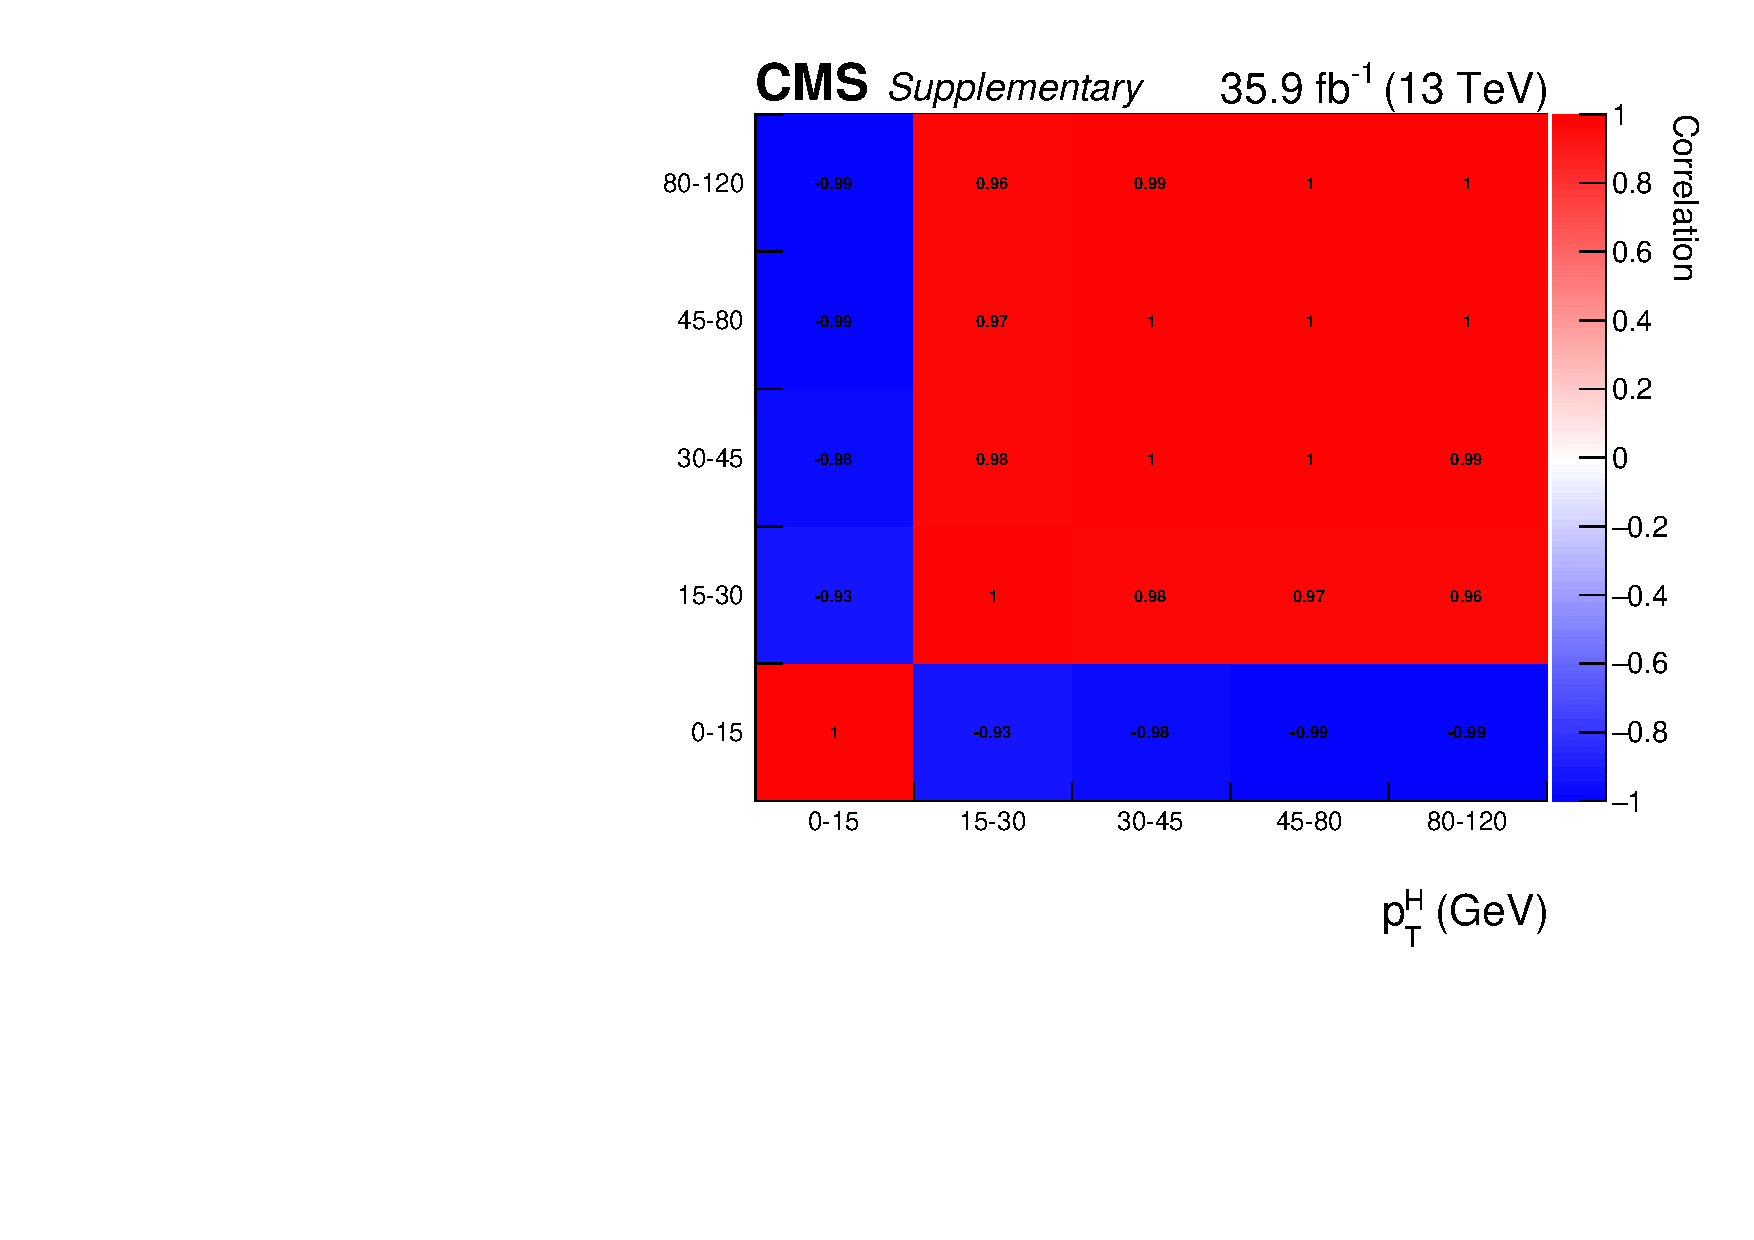
\includegraphics[width=\halflinewidth]{img/interpretation/other/corrmat_yukawa.pdf}
    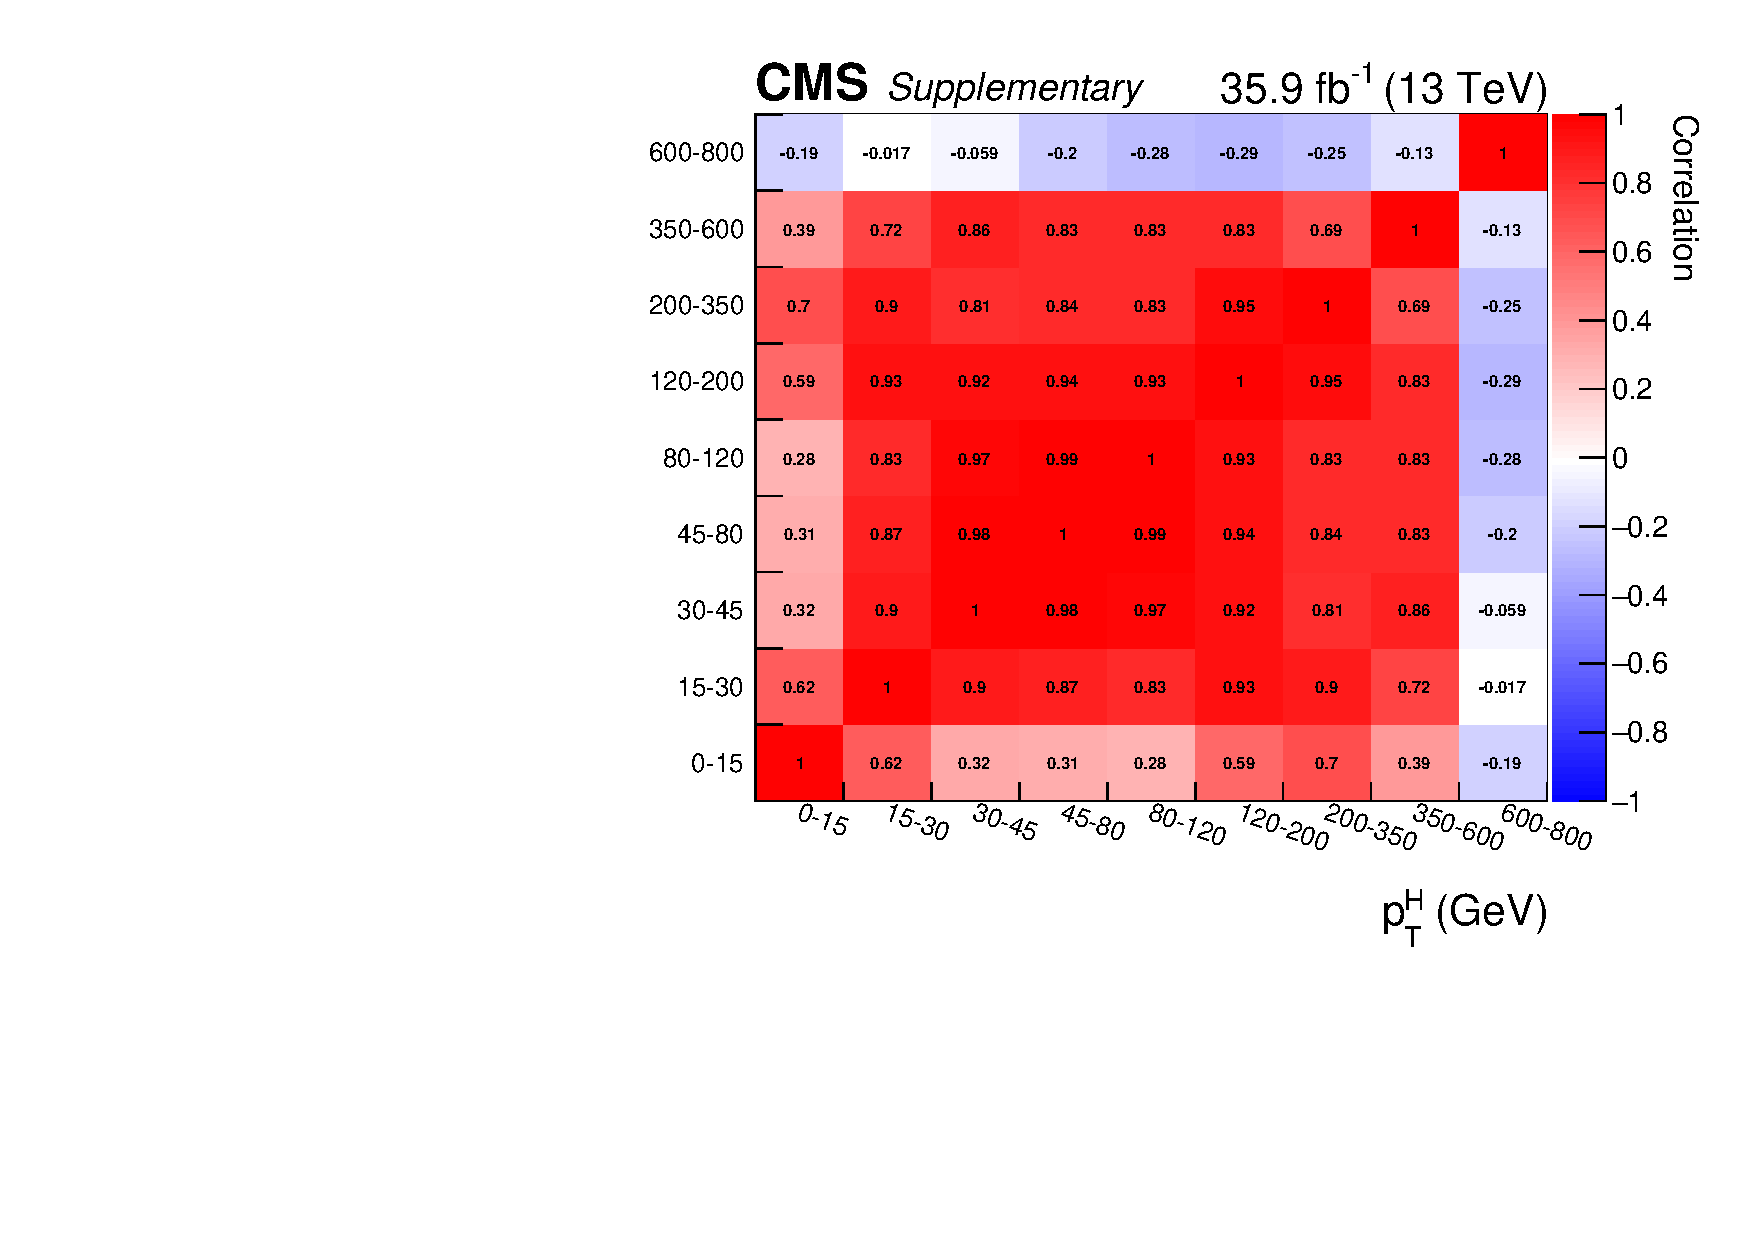
\includegraphics[width=\halflinewidth]{img/interpretation/other/corrmat_tophighpt.pdf}
    \caption{
        Correlation matrices of the scale uncertainties in the experimental $\pth$ binning for the variations of $\kappab$ and $\kappac$ (left), and for the variations of $\kappat$, $\cg$, and $\kappab$ (right).
        }
    \label{fig:scalecorrelationmatrices}
  \end{center}
\end{figure}


In order to assess the resulting correlation structure in more detail, the correlation matrices are produced as well for the finer theoretical binning.
% 
This is achieved by omitting the piecewise integration of the scale variations to the experimental binning.
% 
The resulting correlation matrices are shown in Fig.~\ref{fig:scalecorrelationmatrices-theory}.
% 
For the variations of $\kappab$ and $\kappac$ the observed pattern matches the one from the experimental binning.
% 
For the variations of $\kappat$, $\cg$, and $\kappab$, it now becomes apparent that the bin-to-bin correlations are strongly positive up to roughly $300$\GeV, at which point the finite top mass corrections reduce the correlation with the preceding bins (as expected, since the theoretical calculation becomes significantly different).


\begin{figure}[hbtp]
  \begin{center}
    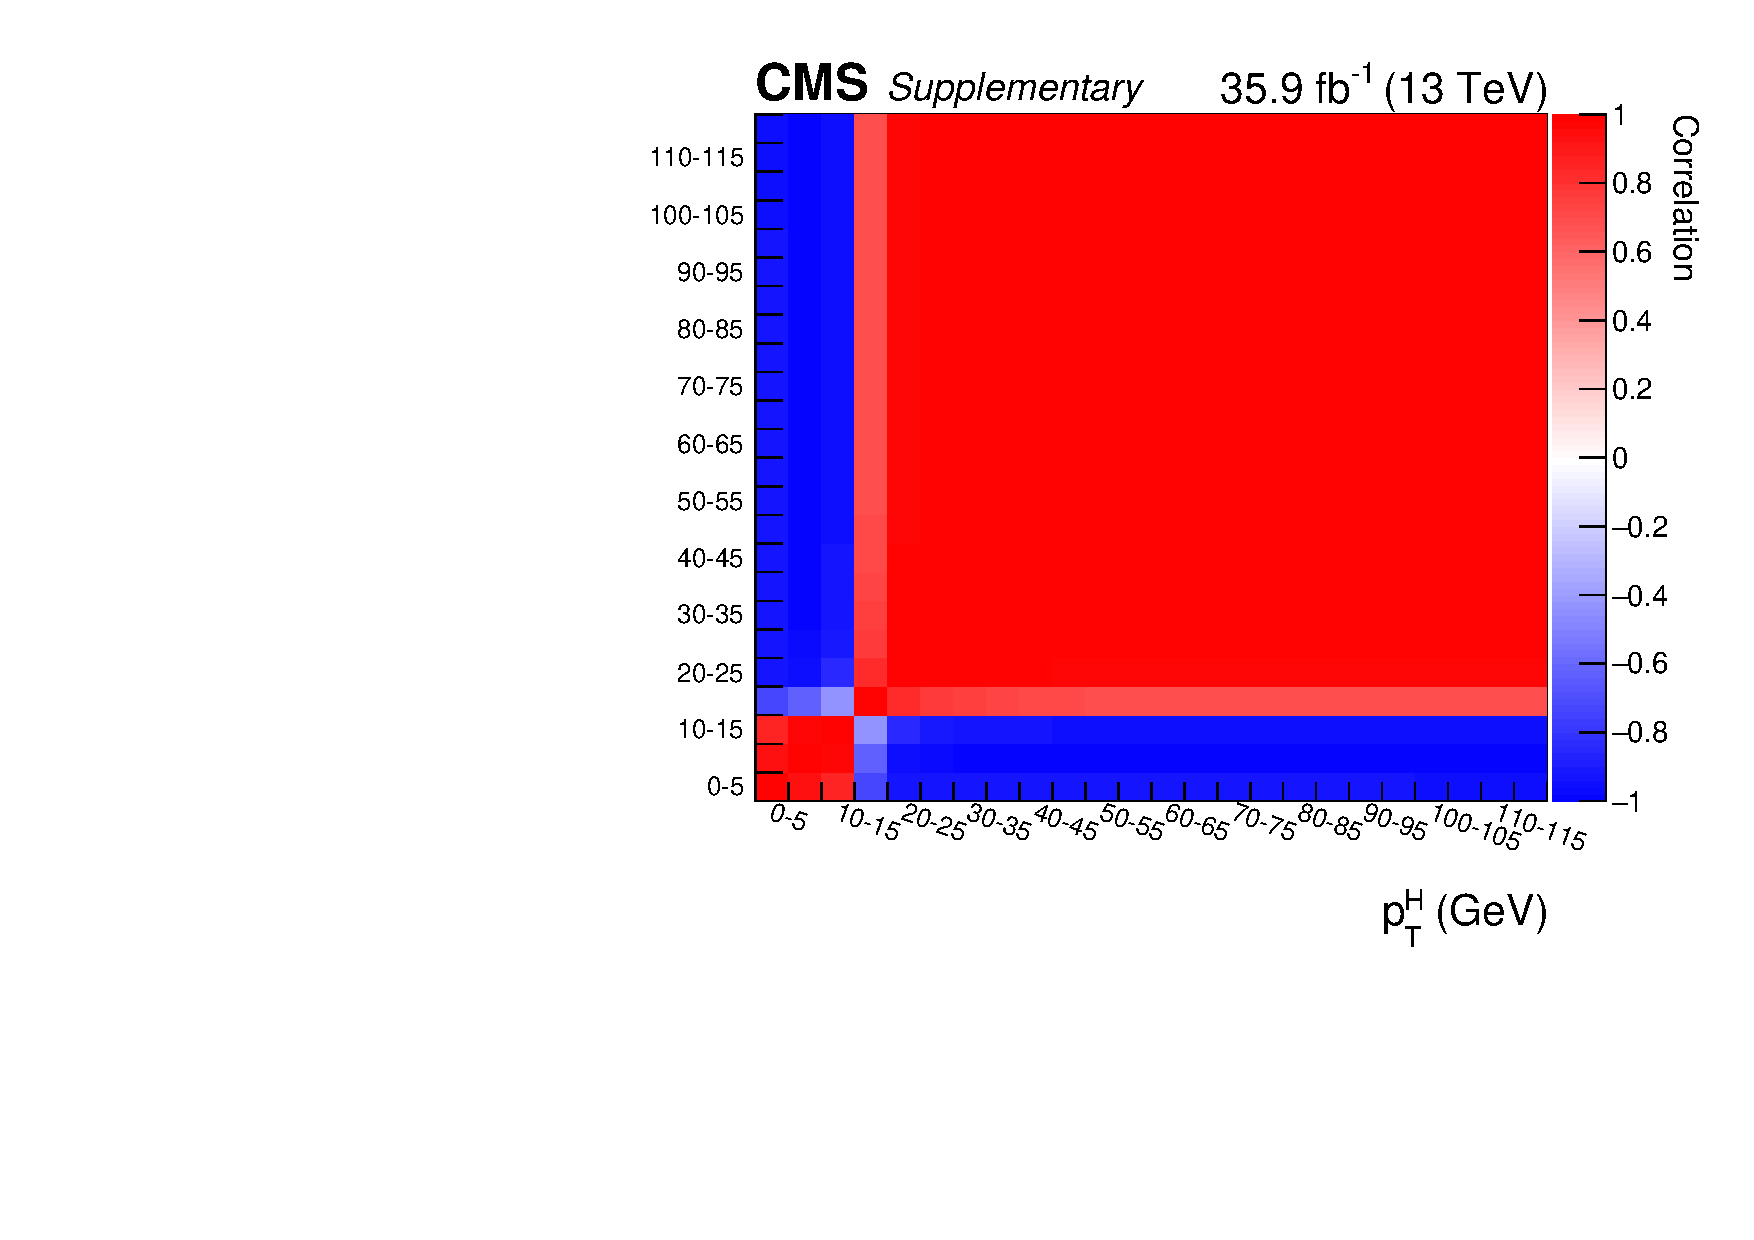
\includegraphics[width=\halflinewidth]{img/interpretation/other/corrmat_theorybinning_yukawa.pdf}
    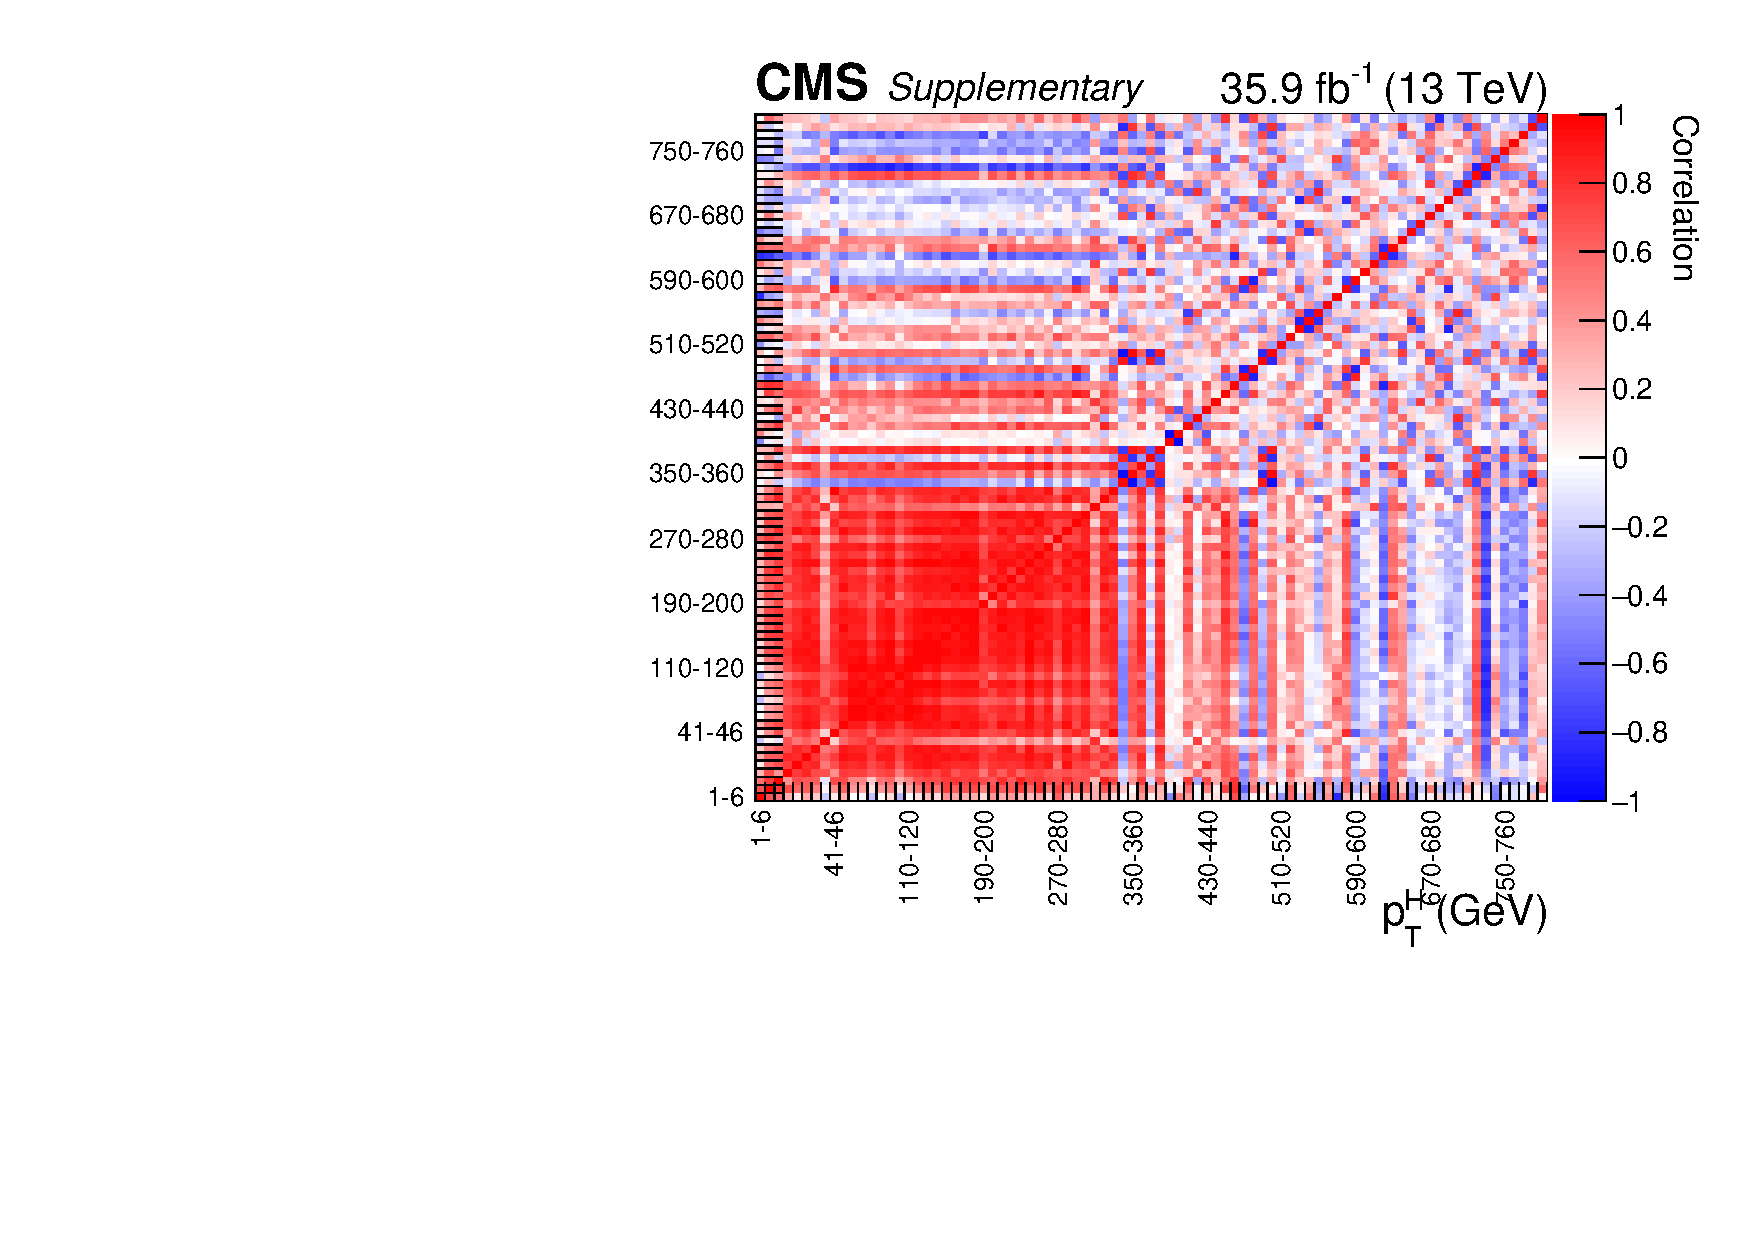
\includegraphics[width=\halflinewidth]{img/interpretation/other/corrmat_theorybinning_tophighpt.pdf}
    \caption{
        Correlation matrices of the scale uncertainties in the $\pth$ binning used for the theoretical calculations for the variations of $\kappab$ and $\kappac$ (left), and for the variations of $\kappat$, $\cg$, and $\kappab$ (right).
        % 
        The numerical values are omitted and the binning is only specified for a limited number of bins in order to avoid overcrowding the plot.
        }
    \label{fig:scalecorrelationmatrices-theory}
  \end{center}
\end{figure}


The effect of the adopted procedure on the results of the interpretation is assessed by performing the same interpretation under three scenarios: The bin-to-bin correlations as described above, no bin-to-bin correlations (i.e. no off-diagonal components in the correlation matrix), and no theoretical uncertainties whatsoever.
% 
With respect to the uncorrelated scale uncertainties (no theoretical uncertainties whatsoever), the adopted procedure increases the overall uncertainty of the interpretation by about $1\%$ ($5\%$).
% 
Thus, while the adopted procedure may lack solid theoretical underpinning, it seems from first principles better motivated than uncorrelated uncertainties, and the effect on the overall uncertainty is rather limited.


Finally, there is no a priori reason for the bin-to-bin correlation structure to be invariant with respect to variations of the Higgs boson couplings.
% 
In order to investigate the effect of coupling variations on the correlation matrix, the correlation matrix is recalculated according to the procedure described above, for a range of variations of $\kappab$ and $\kappac$.%
% 
\footnote{%
Variations of all combinations of $\kappab \in -2, -1, 0, 1, 2$ and $\kappac \in -10, -5, 0, 1, 5, 10$ are considered.
% 
Only the gluon-induced contributions are considered, as only for these contributions the scale variations are calculated for each variation of the couplings.
}
% 
From the resulting set of correlation matrices, the minimum and maximum entries per bin are selected, and are plotted in Fig.~\ref{fig:corrmat-minmax}.
% 
The moderate $\pth$ region is insensitive to variations of the couplings, whereas there is some dependence on the lower $\pth$ region.
% 
Given that the adopted procedure yields only a $1\%$ larger overall uncertainty with respect to no bin-to-bin correlations at all (see above), the effects of the coupling dependence in low $\pth$ bins is neglected in the results that follow.


\begin{figure}[hbtp]
  \begin{center}
    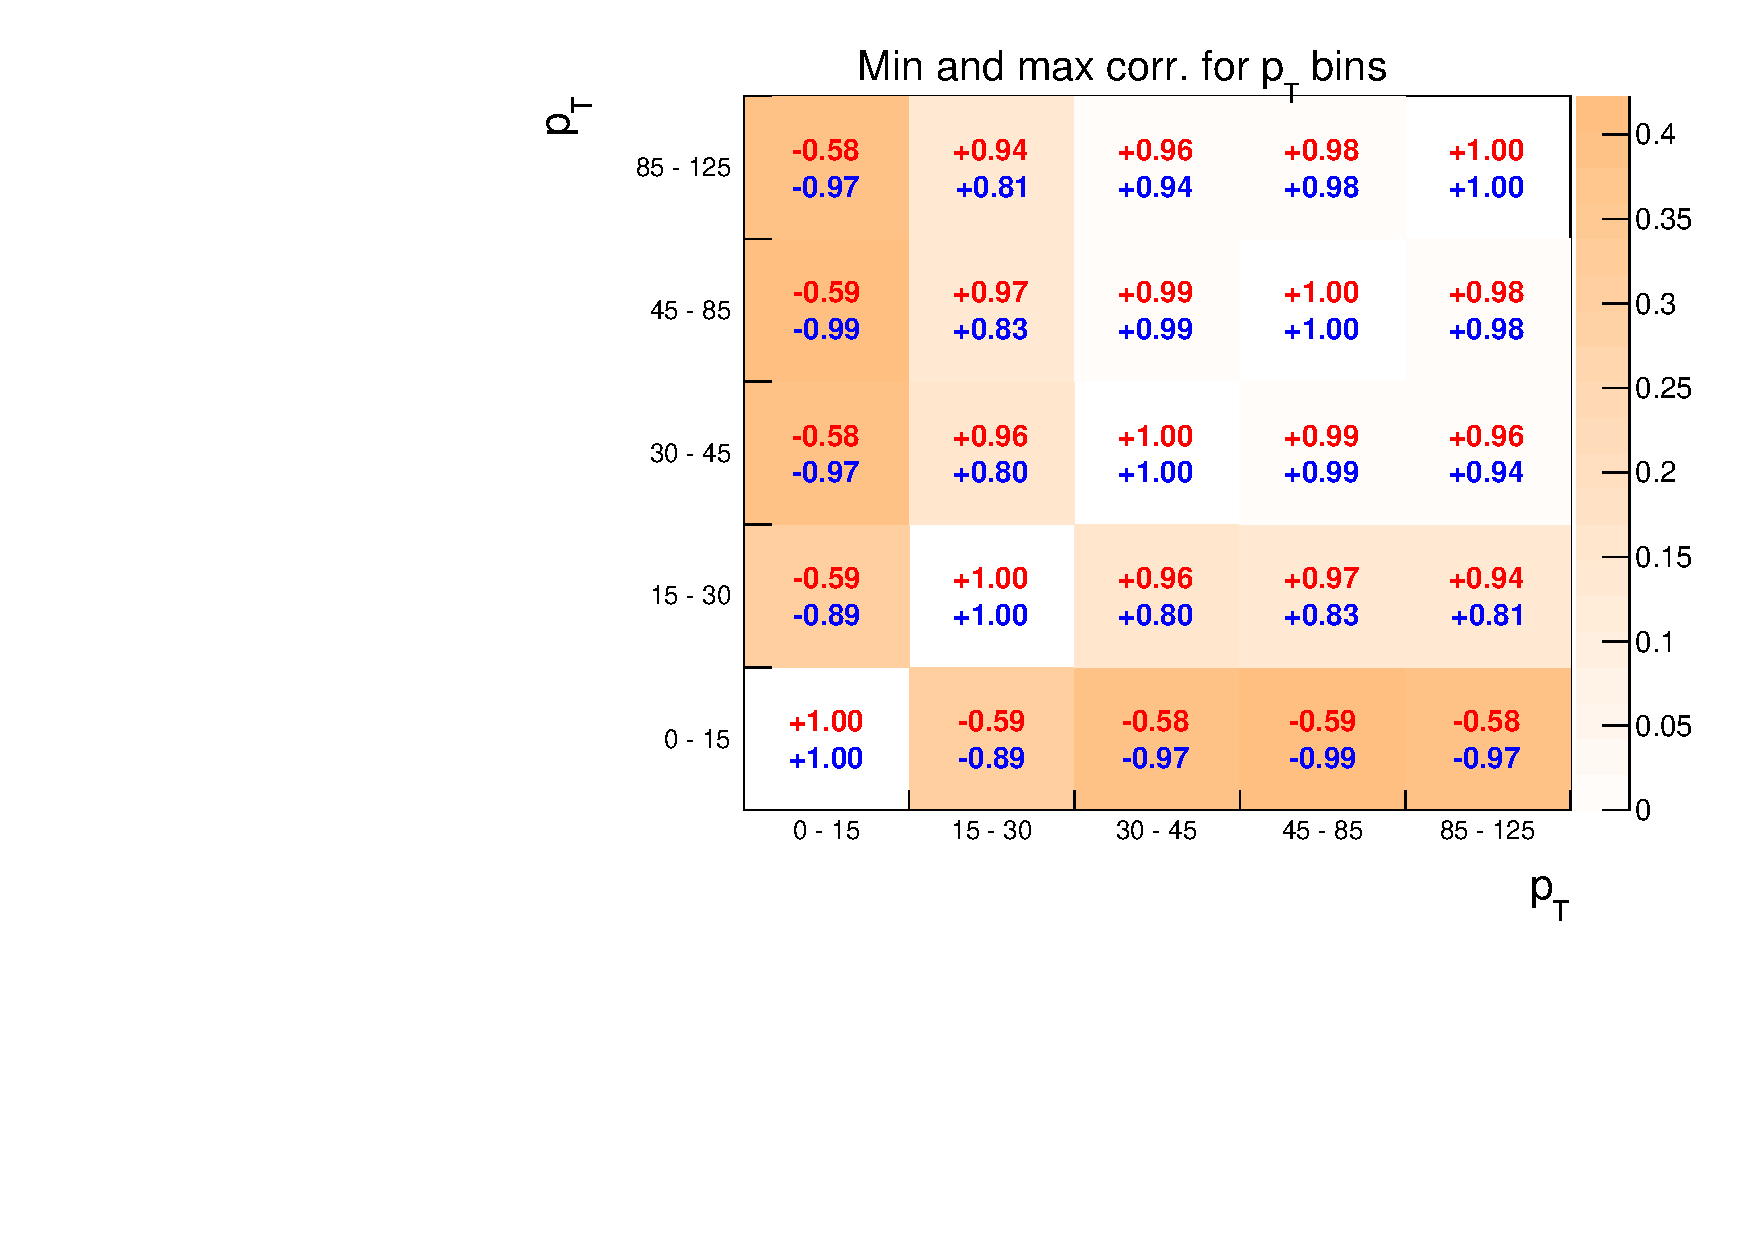
\includegraphics[width=\halflinewidth]{img/interpretation/other/minmax_corrMat_exp.pdf}
    \caption{
        Minima (blue) and maxima (red) of the correlation matrices computed per coupling variation of $\kappa_b$ and $\kappa_c$, for the gluon-induced contributions.
        % 
        The cell color shading corresponds to the difference between the minimum and maximum.
        }
    \label{fig:corrmat-minmax}
  \end{center}
\end{figure}



% ____________________________________________________________________________
% Branching fractions

\subsubsection{Branching fractions}

Some of the interpretations in Sections~\ref{sec:interpretation-results-ktcgkb} and \ref{sec:interpretation-results-kbkc} are based on a SM prescription of branching fractions as functions of the Higgs couplings (see also Section~\ref{sec:interpretation-brs}).
% 
These fits are in principle subject to theoretical uncertainties in the branching fractions, stemming from input parameters of the branching fraction calculation ($\as$, $\mb$, $\mc$ and $\mt$) and missing higher order contributions in the calculations of the partial decay widths.
% 
The impact of these theoretical uncertainties on the interpretation results are assessed.


The uncertainties from missing higher order contributions are assumed to be uncorrelated, whereas the parametric uncertainties are assumed to be fully correlated.
% 
Uncertainties on the partial widths are taken from Ref.~\cite{deFlorian:2016spz}.
% 
Figure~\ref{fig:kbkc-brcomparison} shows the expected simultaneous fit result of $\kappab$ and $\kappac$ with branching fractions fixed to their SM expectation, with and without the uncertainties on the branching fractions.
% 
The theoretical uncertainties on the branching fractions have a clearly negligible impact on the overall interpretation uncertainty, and are thus not further taken into account.


\begin{figure}[hbtp]
  \begin{center}
    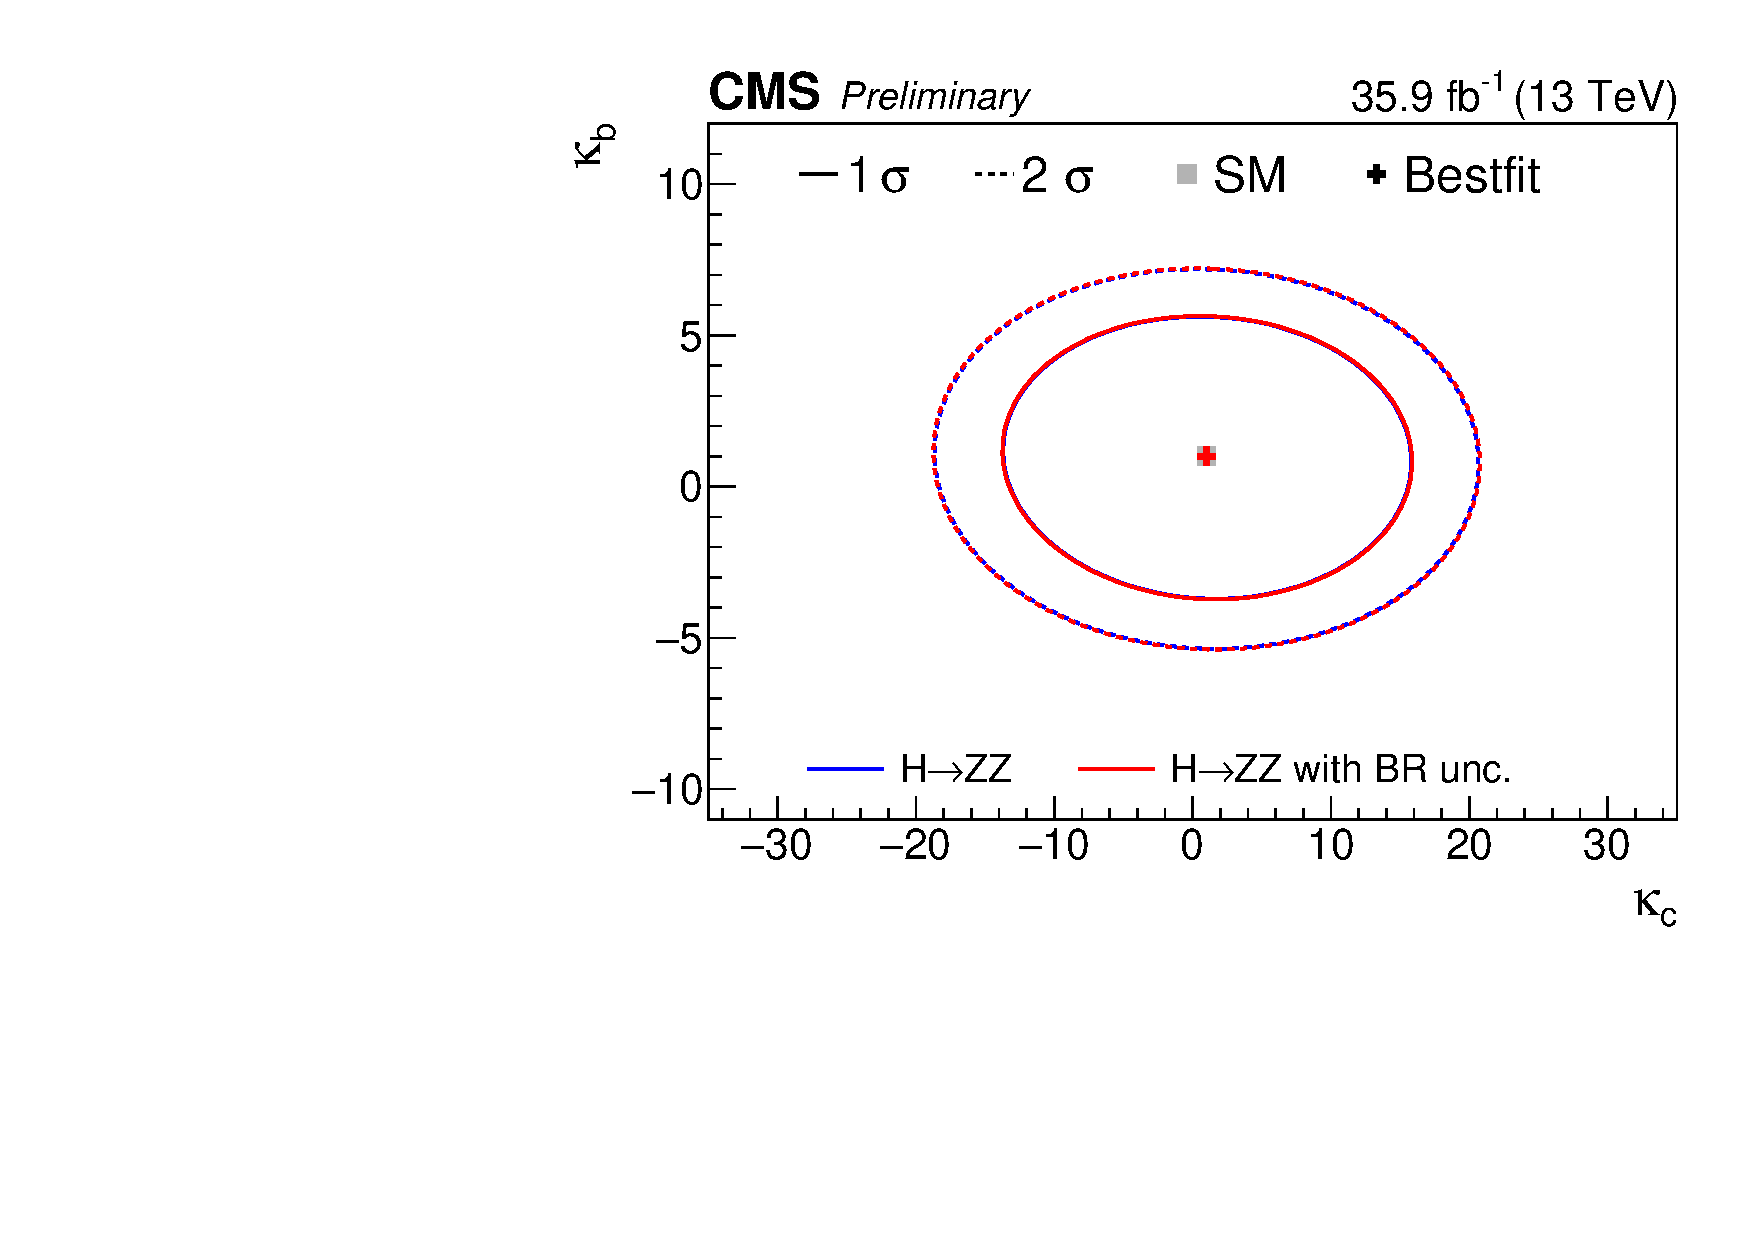
\includegraphics[width=\halflinewidth]{img/interpretation/other/multicont_Yukawa_compareBRuncertainties_asimov.pdf}
    % 
    \caption{
        Expected simultaneous fits of $\kappab$ and $\kappac$ to the differential $\pth$ spectrum using only the $\hzz$ channel, with (red) and without (blue) the branching fraction uncertainties.
        % 
        The branching fractions were fixed to their SM expected value.
        % 
        While the uncertainty is numerically confirmed to be slightly larger when branching fraction uncertainties are taken into account, the overall impact is very small.
        }
    \label{fig:kbkc-brcomparison}
  \end{center}
\end{figure}

